\subsection{Disjoint-probe multilingual revision}
The completed six-method, four-holdout, five-seed revision uses fixed test records and separate training probes and threshold-validation examples. Table~\ref{tab:revision-multieurlex} reports language-average and worst-language outcomes.

\begin{table}[t]
\caption{Completed 120-run language-transfer revision. Each seed contributes a mean and minimum across four independently held-out target languages; entries report mean and seed SD.}
\label{tab:revision-multieurlex}
\centering
\small
\resizebox{\linewidth}{!}{%
\begin{tabular}{lrrrr}
\toprule
Method & Mean micro F1 & Worst micro F1 & Macro F1 & Brier \\
\midrule
FedAvg & 0.337 $\pm$ 0.015 & 0.273 $\pm$ 0.037 & 0.168 $\pm$ 0.010 & 0.184 $\pm$ 0.006 \\
FedProx & 0.335 $\pm$ 0.014 & 0.272 $\pm$ 0.037 & 0.167 $\pm$ 0.010 & 0.185 $\pm$ 0.006 \\
$\lambda=0$ & 0.337 $\pm$ 0.015 & 0.273 $\pm$ 0.037 & 0.168 $\pm$ 0.010 & 0.184 $\pm$ 0.006 \\
Proxy-FLEN & 0.336 $\pm$ 0.017 & 0.276 $\pm$ 0.036 & 0.169 $\pm$ 0.009 & 0.185 $\pm$ 0.006 \\
Local only (target labels) & 0.468 $\pm$ 0.011 & 0.449 $\pm$ 0.013 & 0.163 $\pm$ 0.011 & 0.121 $\pm$ 0.001 \\
Frozen backbone + head & 0.310 $\pm$ 0.013 & 0.256 $\pm$ 0.037 & 0.163 $\pm$ 0.009 & 0.214 $\pm$ 0.016 \\
\bottomrule
\end{tabular}
}
\end{table}


Relative to FedAvg, proxy-FLEN changes average micro-$F_1$ by $-0.11$ points (95\% paired interval $[-0.64,0.43]$) and worst-language micro-$F_1$ by $+0.30$ points (95\% paired interval $[-0.13,0.73]$). The frozen-backbone reference changes average micro-$F_1$ by $-2.68$ points (95\% paired interval $[-3.96,-1.41]$); target-supervised local-only adaptation changes it by $+13.06$ points (95\% paired interval $[11.91,14.21]$). The zero-conflict control reproduces FedAvg. Proxy-FLEN's average contrast spans zero, so the study provides no stable incremental benefit from proxy conflict weighting. Target-language supervision remains substantially stronger than three-round source-language transfer. The frozen-backbone reference trains a classification head and therefore measures the contribution of backbone adaptation.

\begin{figure}[t]
\centering
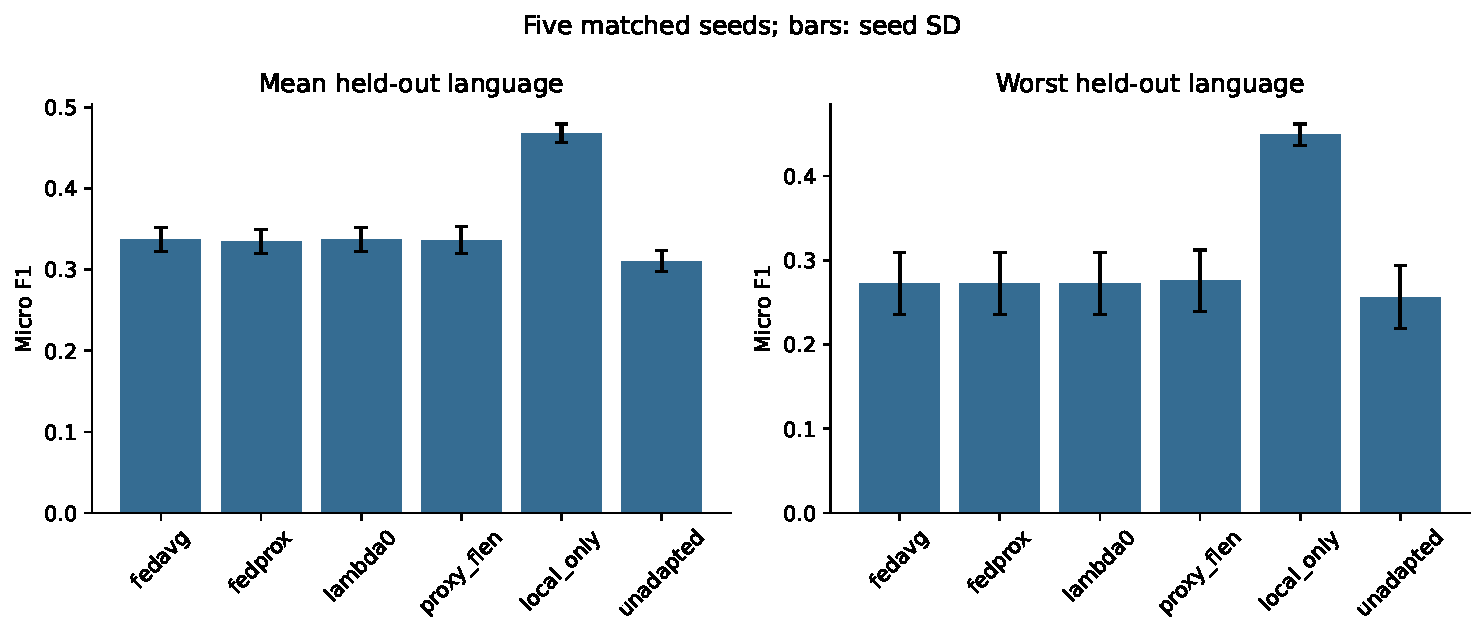
\includegraphics[width=\linewidth]{revision_multieurlex.pdf}
\caption{Mean and worst held-out-language performance in the completed revision; error bars show five-seed SD.}
\label{fig:revision-multieurlex}
\end{figure}
